\documentclass[12pt,onecolumn,a4paper,fleqn]{article}
\usepackage{epsfig,graphicx,subfigure,amsthm,amsmath}
\usepackage[table,xcdraw,svgnames]{xcolor}
\usepackage{setspace}
\usepackage{mathtools}
\usepackage{fancyhdr}
\usepackage{sidecap}
\usepackage{tikz}
\usepackage{pgfplots}
\usetikzlibrary{decorations.pathreplacing}
\usepackage{relsize}
\usepackage{color,xcolor}
\usepackage[framed,numbered]{matlab-prettifier}
\usepackage{files/persianheader}     
\usepackage{float}
\usepackage{enumerate}
\usepackage{booktabs}
\usepackage{setspace}
\usepackage{datetime}
\usepackage{xepersian}


\settextfont[Path=fonts/,BoldFont={ZarBd.ttf},BoldFeatures={Scale=0.9}]{BZar.ttf}

%\DeclarePairedDelimiter\ceil{\lceil}{\rceil}
%\DeclarePairedDelimiter\floor{\lfloor}{\rfloor}

\definecolor{vgreen}{RGB}{104,180,104}
\definecolor{vblue}{RGB}{49,49,255}
\definecolor{vorange}{RGB}{255,143,102}

\pagestyle{fancy}
\fancyhf{}
\rhead{\textbf{آزمایشگاه طراحی سیستم‌های دیجیتال}}
\chead{\textbf{گزارش آزمایش اول}}
\lhead{\textbf{\nouppercase{\rightmark}}}
\cfoot{({\thepage})}
\renewcommand{\headrulewidth}{1pt}
\renewcommand{\footrulewidth}{1pt}
\renewcommand{\sectionmark}[1]{\markright{#1}}
\renewcommand{\subsectionmark}[1]{\markright{#1}}
%\newdateformat{monthyeardate}{%
%	\monthname[\THEMONTH], \THEYEAR}

\onehalfspacing
\begin{document}
	%%% title pages
	\large
	\begin{titlepage}
		
		\begin{center}
			\begin{huge}
				\textbf{
					به نام خدا\\
				}
			\end{huge}
			
			\vspace*{1.5cm}
			
\includegraphics[scale=0.9]{source/sharif1.png}\\
			\vspace*{0.5cm}
			\begin{Large}
				\textbf{
					دانشگاه صنعتی شریف\\
					\vspace*{0.25cm}
					دانشکده مهندسی کامپیوتر\\
				}
			\end{Large}
			\vspace*{3cm}
			\begin{huge}
				\textbf{
					آزمایشگاه طراحی سیستم‌های دیجیتال\\
					\vspace*{1.75cm}
				}
			\end{huge}
			
			\begin{Large}
				\textbf{
					آزمایش اول:\\
					طراحی شماتیک مدار ترکیبی\\
				}
			\end{Large}
			
			\noindent\rule[1ex]{\linewidth}{1pt}
			\vspace*{1.5cm}
			\begin{Large}
					محمدجواد هزاره، یاسین موسوی
					
					\vspace*{1.5cm}
%					\textbf{\today}
					\textbf{
					تابستان 1400
					}
			\end{Large}			
		\end{center}
		\thispagestyle{empty}
	\end{titlepage}	
	\pagebreak
	
	\tableofcontents
	\thispagestyle{empty}
	\pagebreak
	\section{مقدمه}
	\subsection{هدف آزمایش}
	هدف کلی آزمایش آشنایی با سیستم طراحی به کمک شماتیک است که ابزارهای
	\lr{CAD}
	در اختیار ما قرار می‌دهند. به طور خاص در این آزمایش هدف پیاده‌سازی سیستمی است که یک عدد چهار رقمی
	\lr{BCD}
	را ورودی گرفته و با توجه به یک سیگنال ورودی دیگر، تعیین می‌کند که عدد داده شده بر ۳ یا ۱۱ بخش‌پذیر است یا خیر.
	\subsection{تئوری مورد نیاز}
	تئوری مورد نیاز همان قواعد بخش‌پذیری بر ۱۱ و ۳ می‌باشد. می‌دانیم یک عدد بر ۱۱ بخش‌پذیر است اگر و تنها اگر در نمایش ده‌دهی آن ارقام مجاور را یکی در میان با مثبت و منفی علامت‌گذاری کرده و سپس جمع این ارقام را حساب کنیم، حاصل مضربی از ۱۱ باشد. برای بخش‌پذیری بر ۳ نیز می‌دانیم یک عدد بر ۳ بخش‌پذیر است اگر و تنها اگر حاصل جمع ارقام آن بر ۳ بخش‌پذیر باشد.
	
	در این آزمایش برای بخش‌پذیری بر ۱۱ از آن‌چه گفته شد استفاده شده است، و برای بخش‌پذیری بر ۳، علاوه بر آن‌چه که گفته شد، از آن‌چه در ادامه می‌آید نیز استفاده شده است. اگر عدد مورد نظر را به صورت دودویی نمایش دهیم، آنگاه این عدد تنها زمانی بر ۳ بخش‌پذیر خواهد بود که اگر ارقام آن را یکی در میان با مثبت و منفی علامت‌گذاری کرده و سپس جمع این ارقام را حساب کنیم، حاصل مضربی از ۳ باشد. درست مشابه آنچه برای ۱۱ در نمایش ده‌دهی داشتیم.
	\subsection{روش انجام آزمایش}
	با توجه به آن‌چه در قسمت قبل گفته شد، برای پیاده‌سازی سیستم موردنظر و بخش‌پذیری بر هر یک از اعداد به صورت زیر عمل می‌کنیم: (نمای کلی مدار در شکل
	\ref{topModule}
	آمده است.)
	\begin{itemize}
		\item \textbf{بخش‌پذیری بر ۱۱}:
		نخست ارقام اول و سوم را با هم و ارقام دوم و چهارم را با یکدیگر جمع می‌کنیم. سپس حاصل جمع دوم را از اولی کم می‌کنیم و بررسی می‌کنیم که عدد بدست آمده مضربی از ۱۱ است یا خیر. دقت کنیم که در این‌جا به دلیل آن‌که ارقام عدد ورودی، بین ۰ تا ۹ هستند، عدد بدست آمده اگر بخواهد مضربی از ۱۱ باشد، حتما از بین اعداد ۰، ۱۱، و یا منفی ۱۱ خواهد بود.
		\item \textbf{بخش‌پذیری بر ۳}:
		مراحل این قسمت تا جمع کردن اعداد اول و سوم با یکدیگر و اعداد دوم و چهارم با یکدیگر یکسان است. پس از آن در این قسمت این اعداد را با هم جمع می‌کنیم. حال عددی داریم که حاصل جمع ارقام عدد ورودی‌ است. برای بخش‌پذیر بودن عدد ورودی بر ۳، این حاصل جمع باید بر ۳ بخش‌پذیر باشد. در این قسمت از آن‌چه برای بخش‌پذیری بر ۳ در نمایش دودویی اعداد گفته شد استفاده می‌کنیم و به راحتی می‌توان تشخیص داد که عدد بدست آمده بر ۳ بخش‌پذیر است یا خیر.
	\end{itemize} 
	\begin{figure}[H]
		\centering
		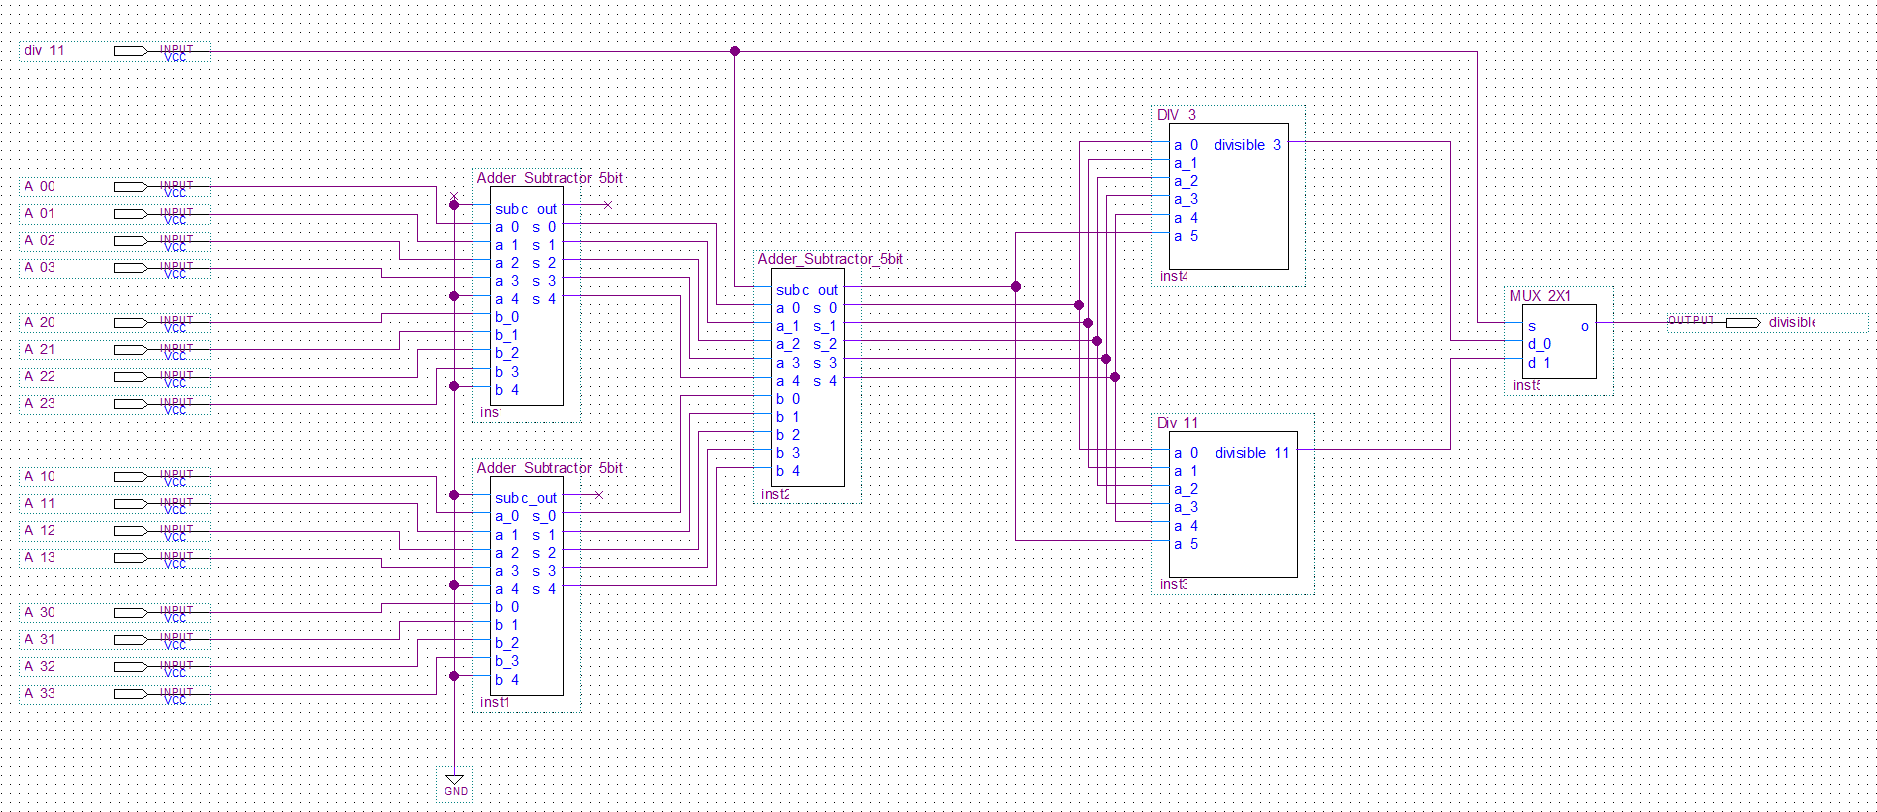
\includegraphics[scale=0.45]{source/top_module.png}
		\caption{نمای کلی سیستم}
		\label{topModule}
	\end{figure}
	\pagebreak
	\section{توصیف معماری مدار}
	
\end{document}